\documentclass[12pt, titlepage]{article}
\usepackage{t1enc}
\usepackage[hungarian, english]{babel}
\usepackage{fancyhdr}
\usepackage{graphicx}
\usepackage{subcaption}

\pagestyle{fancy}


\begin{document}

\fancyhead[R]{Dokumentáció}
\fancyhead[L]{WebTechnológiák}
\selectlanguage{hungarian}
\title{Webtechnológiák féléves beadandó\\Rick and Morty témájú weboldal}
\author{Nagy Balázs EIO1RQ}

\maketitle
\pagebreak

\tableofcontents
\pagebreak

\section*{Bevezetés}
A féléves feladat témájának a népszerű Rick és Morty című Amerikai rajzfilmsorozat került kiválasztásra, mely széleskörű ismeretéből és nagy mennyiségű tartalmából fakadóan lehetővé teszi, hogy változatos módon bemutatásra kerüljön a feladatban adott weboldalon.

\section{Felhasználói felület és oldalak bemutatása}
\subsection{Kezdőoldal - Home}
A weboldal megnyitásakor a felhasználót szembetűnően egy teljes képszélességet elfoglaló borító fogadja, valamint egy rövid leírás a Rick and Morty sorozatról. Itt már érdemes egyből megjegyezni, hogy a teljes weboldal nyelvezete angol és jelen állapotában nem rendelkezik magyar fordítási lehetőséggel.

\begin{figure}[!h]
	\centering
	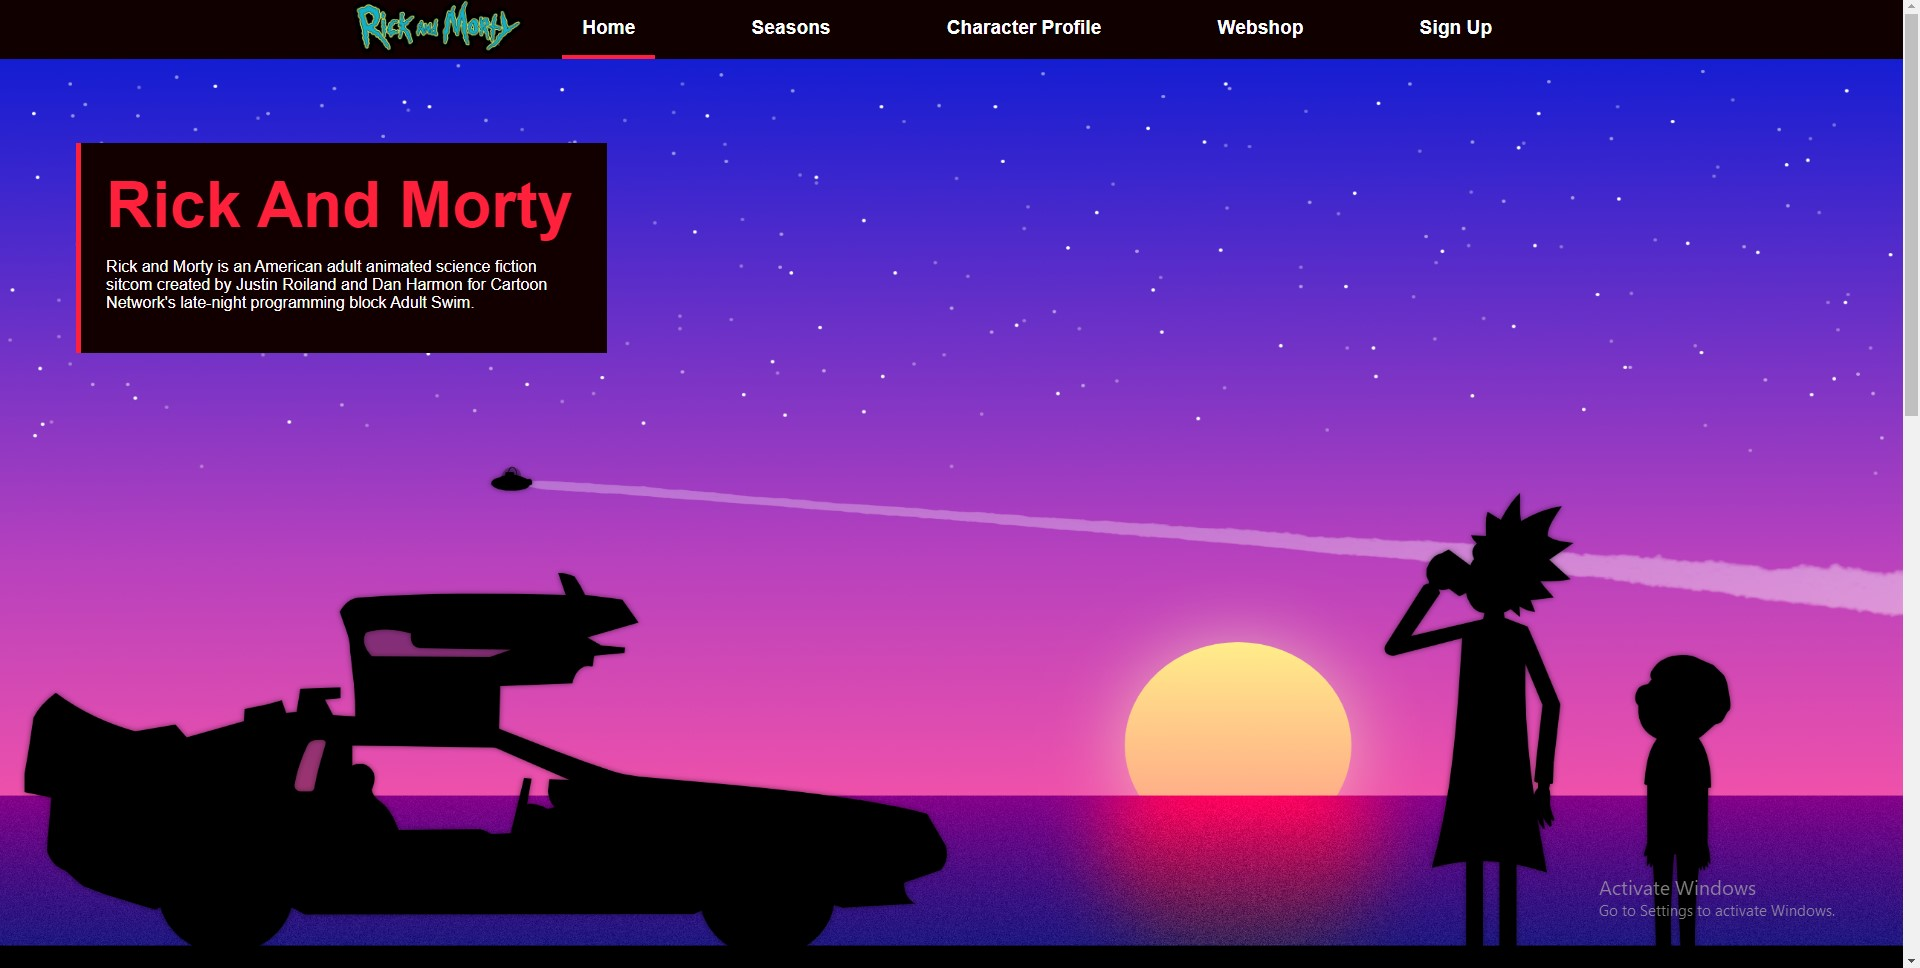
\includegraphics[width=\linewidth]{images/home/1.jpg}
	\caption{Főoldal (1) - Kezdőképernyő}
\end{figure}

\pagebreak

Továbbá, ha a felhasználó lentebb görget, a sorozat első évadának bevezető videója automatikusan elindul és folyamatosan ismétlődik; opcionálisan megállítható. 

\begin{figure}[!h]
	\centering
	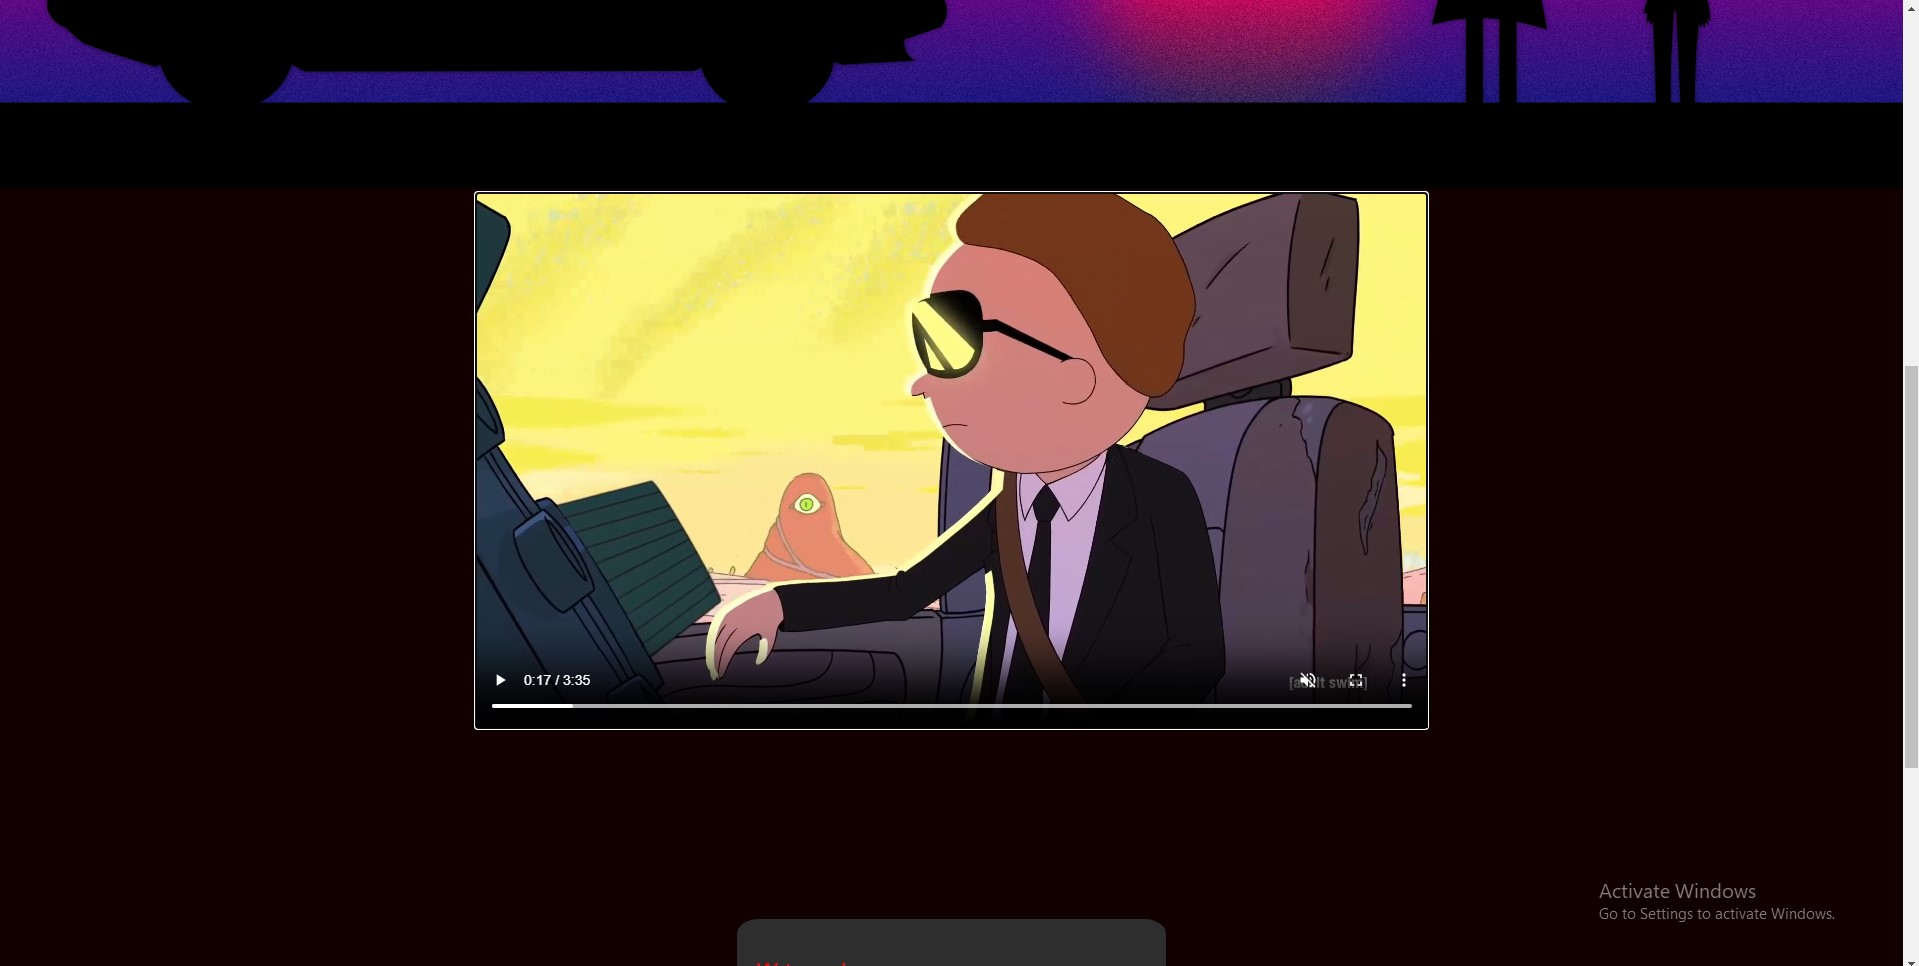
\includegraphics[width=\linewidth]{images/home/2.jpg}
	\caption{Főoldal (2) - Bemutató videó}
\end{figure}

A főoldal legtetejére visszatérve tudunk navigálni az oldal többi részére; piros aláhúzás jelzi, hogy jelenleg az 5 html oldal közül melyiken tartózkodunk éppen.

\begin{figure}[!h]
	\centering
	
\includegraphics[width=\linewidth]{images/home/3.jpg}
	\caption{Főoldal (3) - Navigáció} 
\end{figure}

Ha a navigációs elemek fölött elhúzzuk az egér kurzort, akkor a szöveg piros színűre változik, ezzel jelezve az éppen "kiválasztott" oldalt. Az elemek linkek segítségével működnek.

\begin{figure}[!h]
	\centering
	
\includegraphics[width=\linewidth]{images/home/4.jpg}
	\caption{Főoldal (4) - Kijelölés} 
\end{figure}

\pagebreak
A weboldal legalján egy kapcsolatfelvételre alkalmas rész található, ahol lehetőség van üzenni a támogató személyzetnek; ez csupán esztétikai és technikai demonstrációs okokból kapott helyet.
A form tartalmaz szövegdobozokat az email és üzenet rögzítéséhez, egy check-boxok, ha a felhasználó szeretne visszajelzést kapni, illetve egy  radio button-t is.

\begin{figure}[!h]
	\centering
	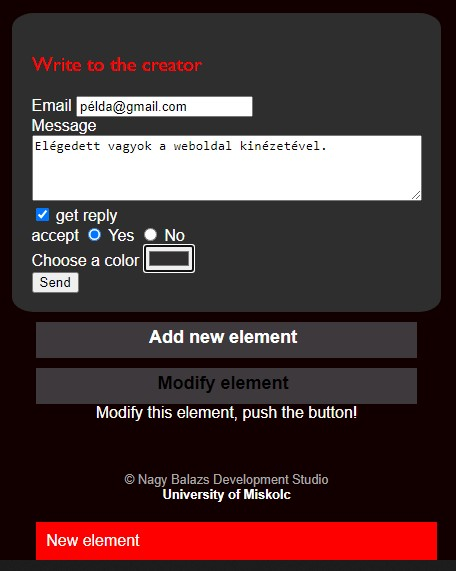
\includegraphics[width=0.7\linewidth]{images/home/5.jpg}
	\caption{Főoldal (3) - Navigáció} 
\end{figure}

\pagebreak
Ezen felül elérhető egy színválasztó elem is technikai demonstráció céljából. Az alsó két gomb szerepe szintén hasonló demonstráció, melyről részletesebben a \textbf{JavaScript} fejezetben lesz szó.

\begin{figure}[!h]
	\centering
	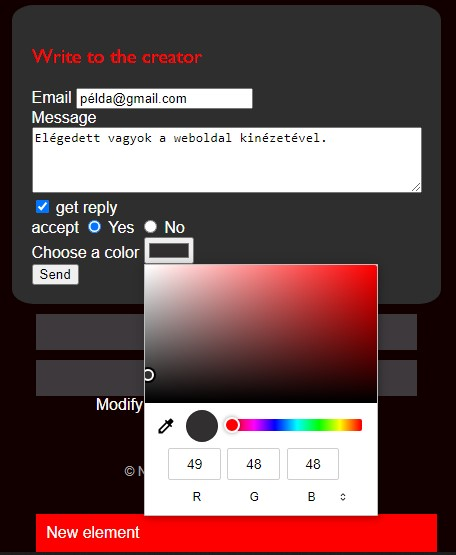
\includegraphics[width=0.7\linewidth]{images/home/6.jpg}
	\caption{Főoldal (3) - Színválasztás} 
\end{figure}

\pagebreak

\subsection{Évadok - Seasons}
Az évadok fül alatt találunk egy rövid és egy részletes felsorolást az elérhető évadokról egyébb hasznos információkkal egybekötve.
A rövid felsorolás számozott, illetve számozatlan listával van megvalósítva.

\begin{figure}[!h]
	\centering
	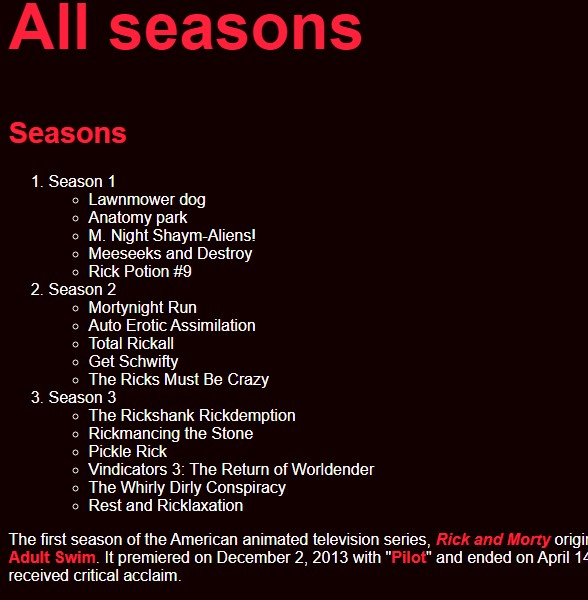
\includegraphics[width=0.6\linewidth]{images/seasons/1.jpg}
	\caption{Évadok (1) - Rövid felsorolás} 
\end{figure}

Egy részletesebb összefoglalás található lentebb, ami táblázatos formában jeleníti meg az adatokat.

\begin{figure}[!h]
	\centering
	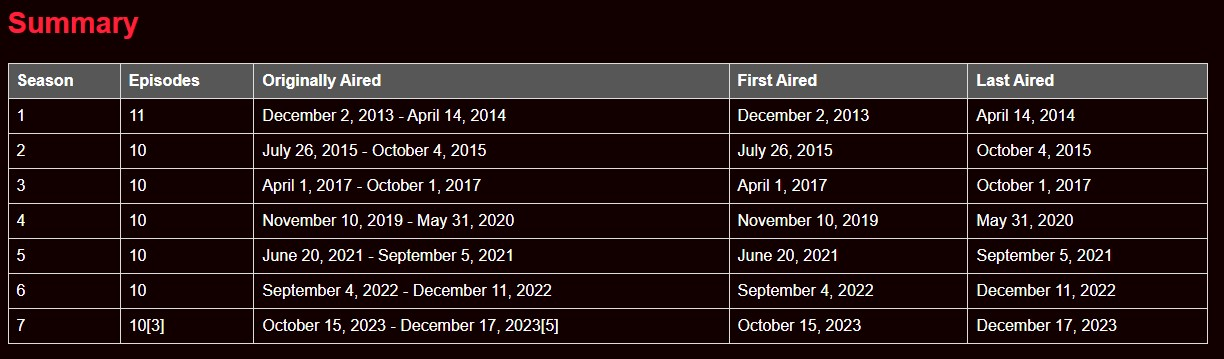
\includegraphics[width=\linewidth]{images/seasons/2.jpg}
	\caption{Évadok (2) - Részletes összefoglalás} 
\end{figure}

Az oldal alján interaktív képek helyezkednek el, amelyek korábbi epizódokból lettek kiválasztva.

\begin{figure}[!h]
	\centering
	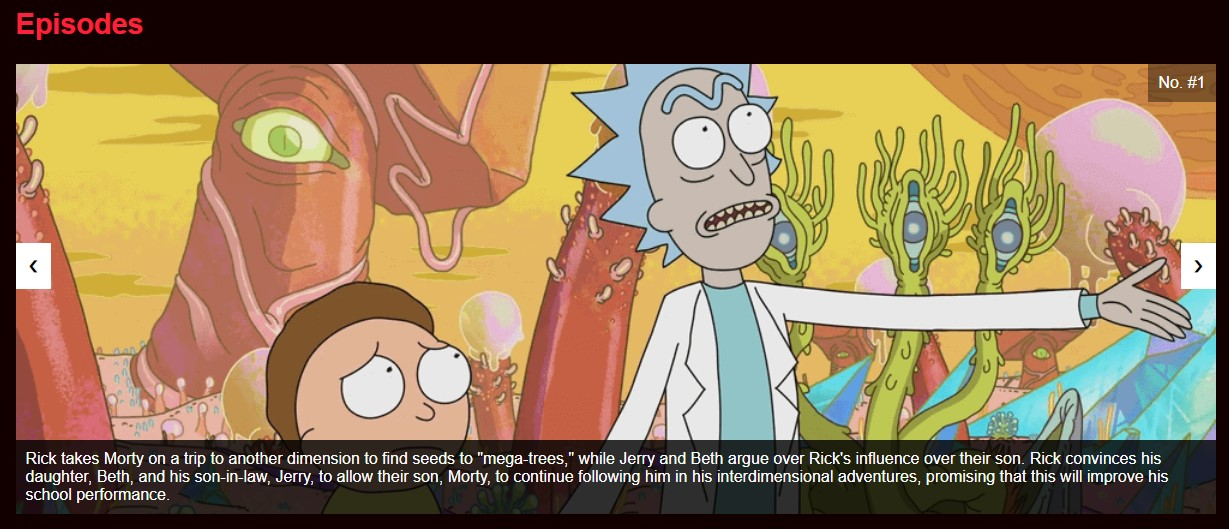
\includegraphics[width=\linewidth]{images/seasons/3.jpg}
	\caption{Évadok (3) - Interaktív képek}
\end{figure}

\begin{figure}[!h]
	\centering
	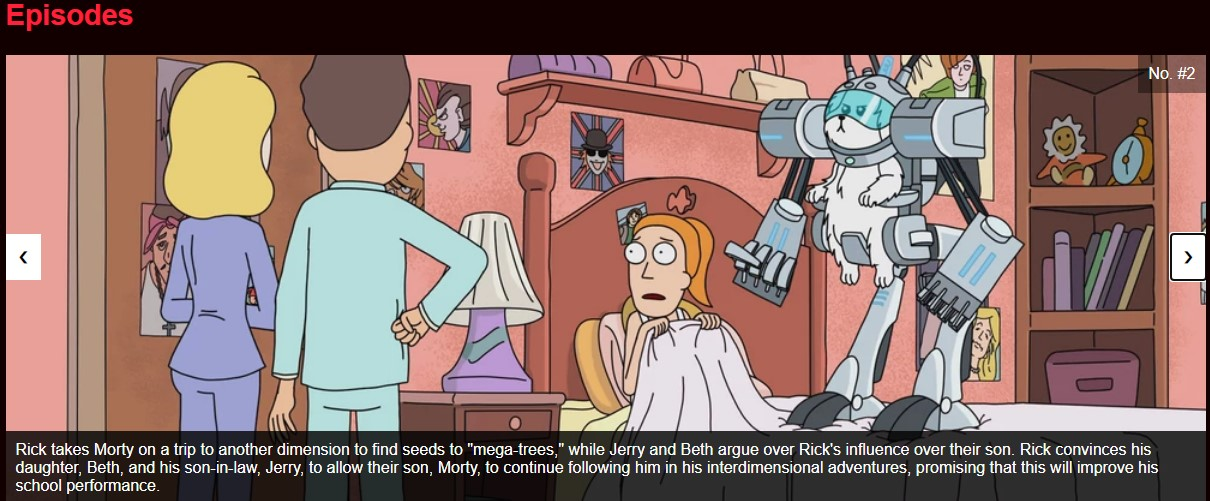
\includegraphics[width=\linewidth]{images/seasons/4.jpg}
	\caption{Évadok (4) - Interaktív képek}
\end{figure}

\pagebreak

\subsection{Szereplők leírása - Character Profile}
Főbb szereplők felsorolása, illetve rövid jellemzése található a fül alatt képekkel ellétva, melyek az előző fejezetben is használt animációk szerint válnak interaktívvá.

\begin{figure}[!h]
	\centering
	
\includegraphics[width=\linewidth]{images/characters/1.jpg}
	\caption{Szereplők leírása (1) - Morty}
\end{figure}

\begin{figure}[!h]
	\centering
	
\includegraphics[width=\linewidth]{images/characters/2.jpg}
	\caption{Szereplők leírása (2) - Morty, kurzor interakcióval nagyítva}
\end{figure}

\pagebreak

\subsection{Webáruház - Webshop}
A felhasználó itt tud rendelni a sorozattal kapcsolatos ajándékfigurákat, ahol az ár euro-ban van felűntetve, valamint szintén a korábbi képekhez hasonló animáció kerül megjelenítésre kurzoros interakció esetén.

\begin{figure}[!h]
	\centering
	
\includegraphics[width=\linewidth]{images/webshop/1.jpg}
	\caption{Webáruház (1) - Ajándék figurák}
\end{figure}

\begin{figure}[!h]
	\centering
	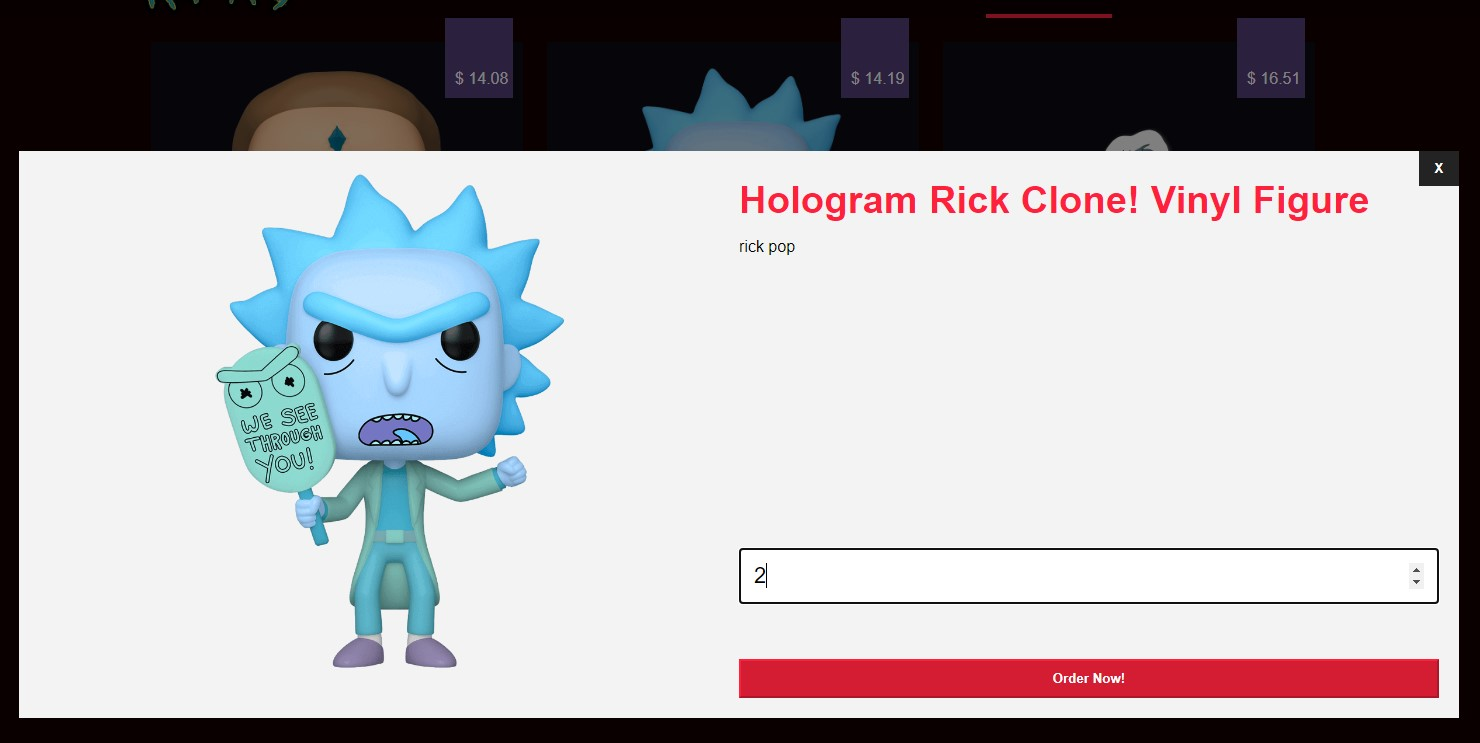
\includegraphics[width=\linewidth]{images/webshop/2.jpg}
	\caption{Webáruház (2) - Rick figura rendelés}
\end{figure}

\pagebreak

\subsection{Regisztráció - Sign Up}
Az oldalra való regisztrálásra is van lehetősége a felhasználonak. Az alábbi formot kell helyesen kitöltenie, ami hiba esetén piros szöveggel és a hibás mező bekeretezésével jelzi a problémát.

\begin{figure}[!h]
	\centering
	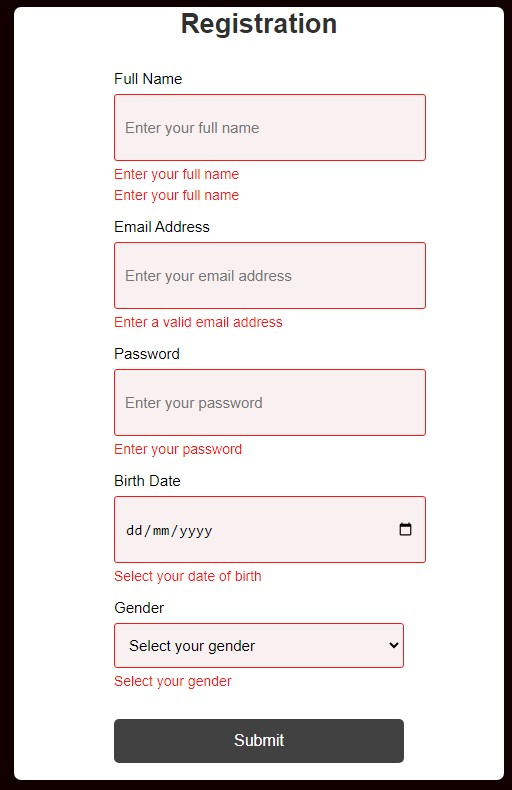
\includegraphics[scale=0.7]{images/signup/1.jpg}
	\caption{Regisztráció (1) - Hibás regisztráció}
\end{figure}

Ellenőrzés és helyes kitöltés után a form nem jelez több hibát; beküldés esetén a mezők üressé válnak, mivel a funkció nincsen implementálva.

\begin{figure}[!h]
	\centering
	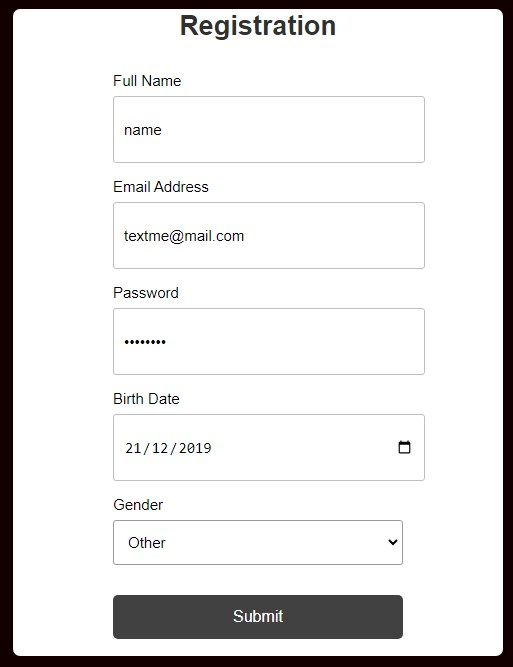
\includegraphics[width=0.7\linewidth]{images/signup/2.jpg}
	\caption{Regisztráció (1) - Helyes regisztráció}
\end{figure}

\pagebreak

\section{Kód bemutatása}
\subsection{HTML}
Összesen 5 darab HTML oldal található a projektben, melyek:
\begin{itemize}
	\item{index.html}
	\item{seasons.html}
	\item{characters.html}
	\item{webshop.html}
	\item{registration.html}
\end{itemize}

Alap HTML elemeket sűrűn tartalmaz a kódbázis, azonban csak a legfontosabbak kerülnek itt említésre demonstrációs okkal.

\begin{figure}[!h]
	\centering
	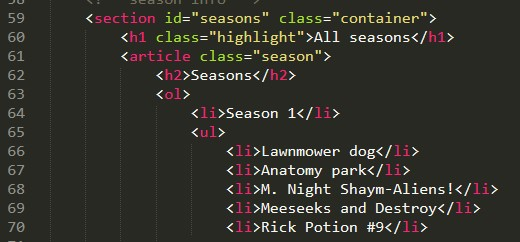
\includegraphics[width=\linewidth]{images/html/1.jpg}
	\caption{Alap HTML elmek (1) - címsorok, listák}
\end{figure}

\pagebreak

\begin{figure}[!h]
	\centering
	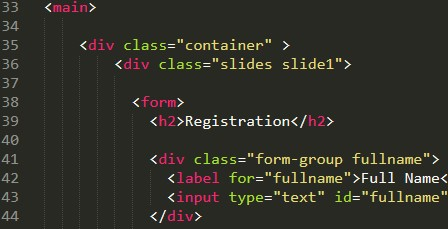
\includegraphics[width=0.9\linewidth]{images/html/2.jpg}
	\caption{Alap HTML elmek (2) - div}
\end{figure}

\begin{figure}[!h]
	\centering
	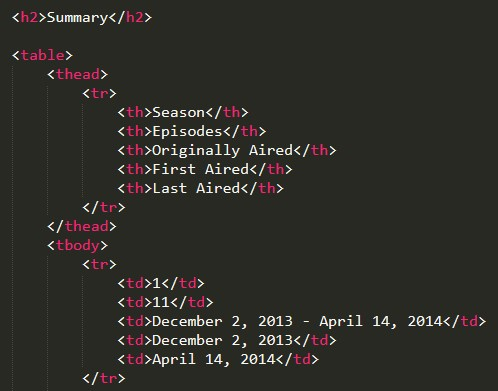
\includegraphics[width=0.9\linewidth]{images/html/4.jpg}
	\caption{Alap HTML elmek (3) - táblázat}
\end{figure}

\begin{figure}[!h]
	\centering
	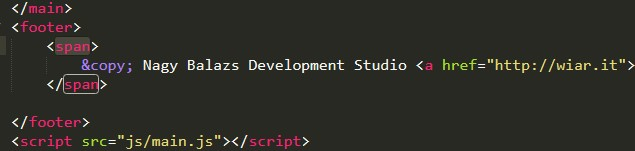
\includegraphics[width=0.8\linewidth]{images/html/3.jpg}
	\caption{Alap HTML elmek (4) - span és link}
\end{figure}

Űrlapok és regisztrációs oldal elemei a forráskódban:

\begin{figure}[!h]
	\centering
	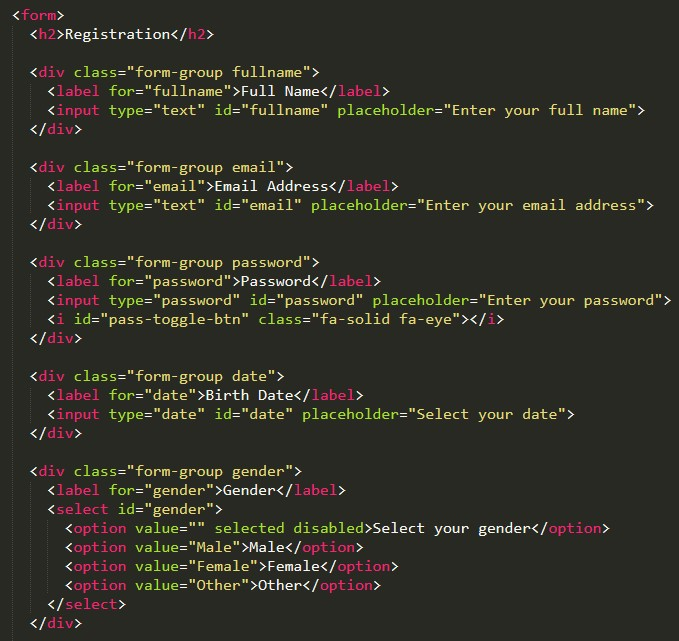
\includegraphics[width=\linewidth]{images/html/5.jpg}
	\caption{Űrlap elemek (1) - Szöveges mezők, email, dátum, opciók}
\end{figure}

\pagebreak
\begin{figure}[!h]
	\centering
	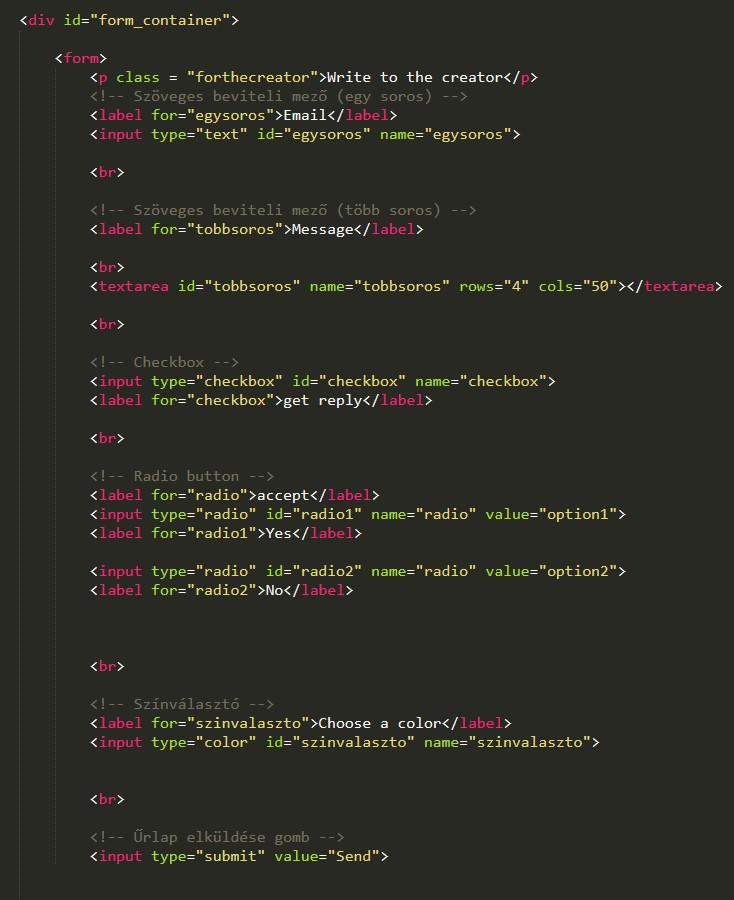
\includegraphics[width=\linewidth]{images/html/6.jpg}
	\caption{Űrlap elemek (2) - text, checkbox, radio button, color}
\end{figure}

\pagebreak


\subsection{CSS}
Az oldal kinézetét egészben definiáló stílus a \textit{main.css} fájlban található, valamint ezen kívül a külön lett választva a regisztrációs form, illetve a responsive felület megjelenéséért felelős kód \textit{registration\_panel.css} és \textit{responsive.css} fájlokba. 

HTML-be beágyzott CSS, azonosító alapján való formázás

\begin{figure}[!h]
	\centering
	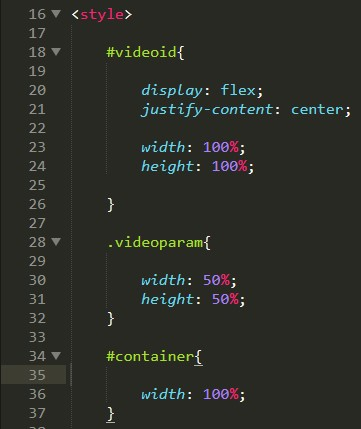
\includegraphics[width=0.8\linewidth]{images/css/1.jpg}
	\caption{CSS formázás (1) - Elemek kiválasztása}
\end{figure}

\pagebreak

Regisztrációs űrlap szerkezeti elemeinek és megjelenésének formázása:
\begin{figure}[!h]
	\centering
	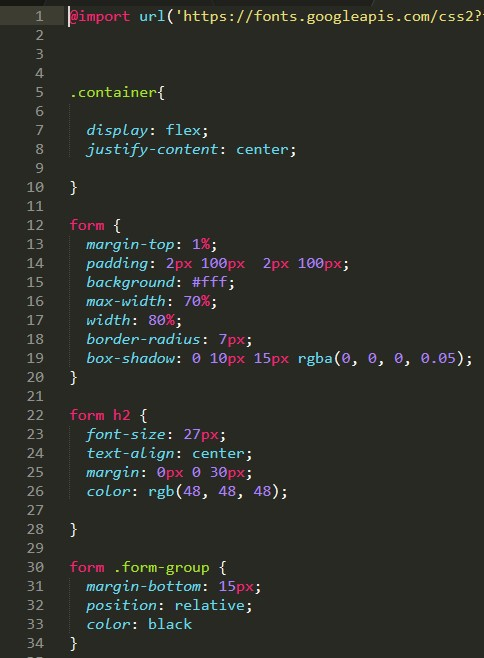
\includegraphics[width=0.8\linewidth]{images/css/2.jpg}
	\caption{CSS formázás (2) - Űrlap}
\end{figure}

\pagebreak

Menü kialakítása
\begin{figure}[!h]
	\centering
	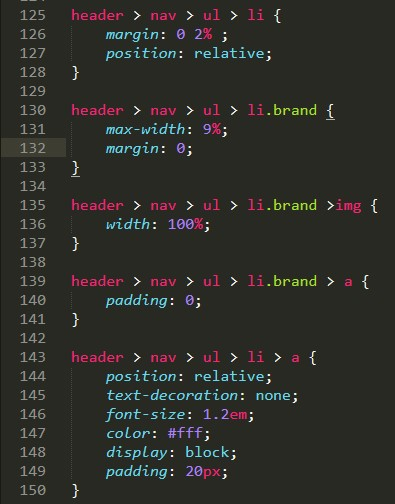
\includegraphics[width=0.8\linewidth]{images/css/3.jpg}
	\caption{CSS formázás (3) - Menü}
\end{figure}

\pagebreak

Linkek
\begin{figure}[!h]
	\centering
	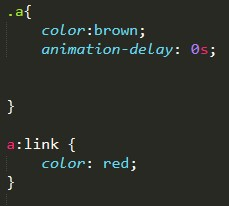
\includegraphics[width=0.6\linewidth]{images/css/4.jpg}
	\caption{CSS formázás (4) - Link}
\end{figure}

Gombok és háttérszín
\begin{figure}[!h]
	\centering
	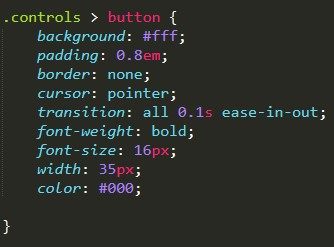
\includegraphics[width=0.6\linewidth]{images/css/5.jpg}
	\caption{CSS formázás (4) - Gomb}
\end{figure}

\pagebreak

\subsection{JavaScript}
Az interakcióért felelős scriptek szintén külön fileokban foglalnak helyet.
A regisztrációs form ellenőrzésére a következő script szolgál:
\begin{figure}[!h]
	\centering
	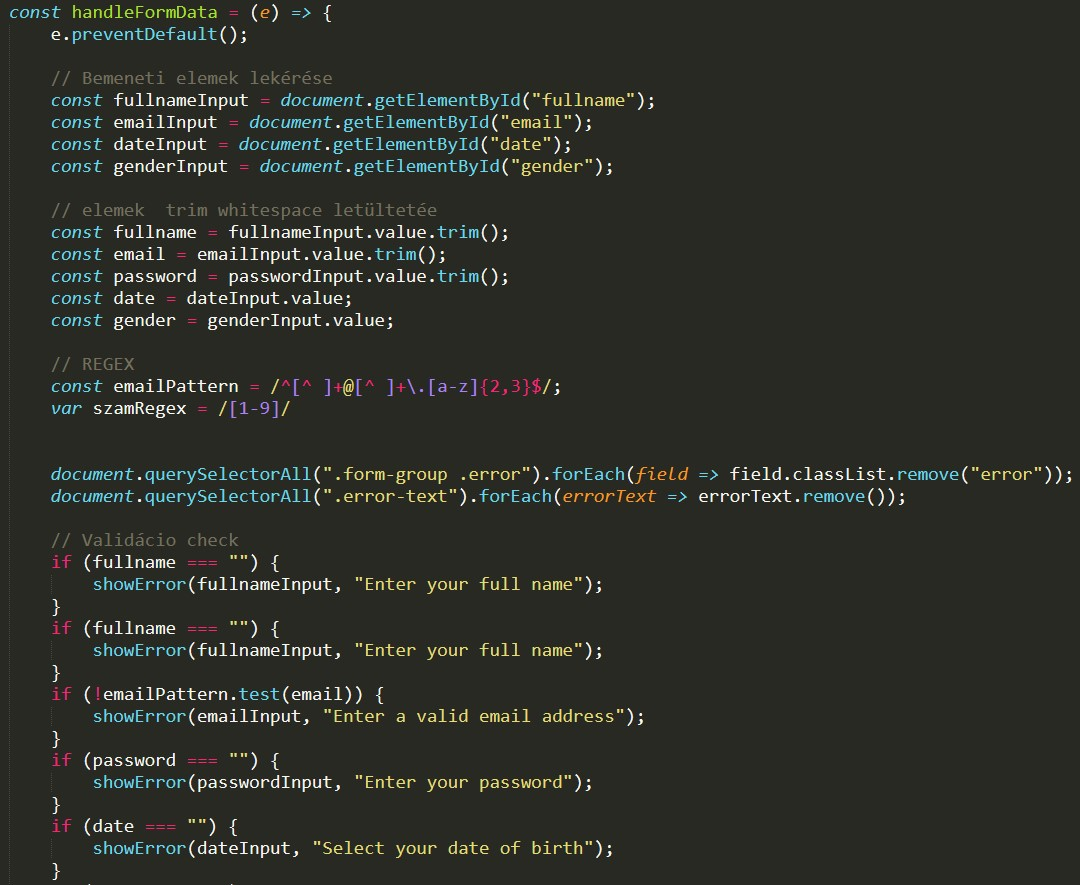
\includegraphics[width=\linewidth]{images/javascript/1.jpg}
	\caption{JavaScript (1) - Ellenőrzés}
\end{figure}

\pagebreak
Az oldalon megtalálható animációk egyike
\begin{figure}[!h]
	\centering
	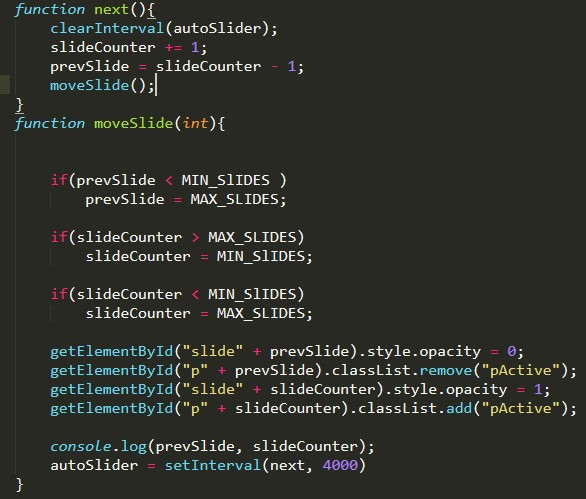
\includegraphics[width=\linewidth]{images/javascript/2.jpg}
	\caption{CSS formázás (2) - Animáció}
\end{figure}

\pagebreak

Új elem készítése és meglévő elem módosítása:
\begin{figure}[!h]
	\centering
	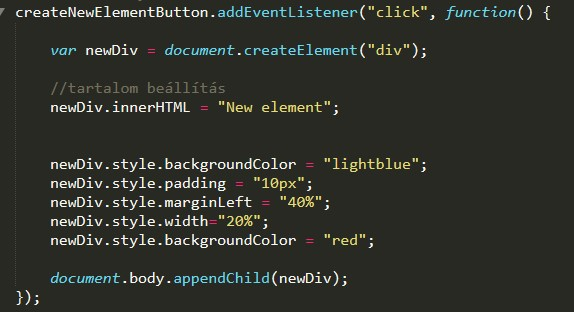
\includegraphics[width=\linewidth]{images/javascript/3.jpg}
	\caption{CSS formázás (4) - Új elem létrehozása}
\end{figure}

\begin{figure}[!h]
	\centering
	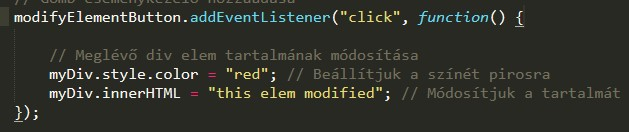
\includegraphics[width=\linewidth]{images/javascript/4.jpg}
	\caption{CSS formázás (4) - Meglévő elem módosítása}
\end{figure}

\end{document}